\documentclass[acmsmall, nonacm]{acmart}

% %%
%% \BibTeX command to typeset BibTeX logo in the docs
\AtBeginDocument{%
  \providecommand\BibTeX{{%
    Bib\TeX}}}

%% end of the preamble, start of the body of the document source.
\begin{document}

\title{Torchlight: Diffusion-based Network Trace Generation from the DARPA Searchlight Dataset}

\author{Ray Zhao}
\affiliation{%
 \institution{University of Southern California}
 \city{Los Angeles}
 \state{California}
 \country{}}
\email{rdzhao@usc.edu}

\author{Alefiya Hussain}
\affiliation{%
  \institution{USC/ISI}
  \city{Los Angeles}
  \country{}}
\email{hussain@isi.edu}

\renewcommand{\shortauthors}{Zhao, Hussain}

\begin{abstract}
  At present, there is a severe lack of both comprehensive and realistic labeled datasets
  for machine learning applications in the networking domain. Predominantly, prior generative
  work has focused on lower-dimensional representations that rely on aggregating flow 
  characteristics and lack the fine-grain of raw network traces. This results in suboptimal
  performance in machine learning contexts and limited applications outside of those 
  contexts. This has induced a push for new generative techniques to provide 
  synthetic data for usage both on its own and layered in with real data as augmentation.
  In this paper, we present Torchlight, a diffusion-based
  generation framework built atop and extending techniques first introduced in 
  \textit{NetDiffusion} \cite{Jiang2024} using DARPA Searchlight \cite{Ardi2022} data to generate synthetic network traces
  for video streaming applications. We demonstrate the efficacy of Torchlight in generating
  synthetic network traces that reasonably resemble real-world data and perform notably well
  in classification tasks. 
\end{abstract}

\maketitle

\section{Introduction}
There's a large need and general scarcity of labeled network datasets,
as high-quality data is often expensive and frought with privacy concerns,
and the datasets that do exist are often left rarely update over time.
Synthetic data generation techniques aim to solve this problem, but prior
GAN based methodologies have been limited in their ability to generate
raw, high-dimensional traces and often rely on aggregating flow characteristics,
which results in data that lacks statistical fidelity to real data and performs
much more poorly in machine learning tasks. The highly specific formatting of
these types of condensed traces also renders them generally incompatible with
traditional tools like Wireshark and tcpdump.

In recent years, the advent of diffusion models have solved many of the
problems that plague older GAN frameworks, being able to capture much
more complex patterns and relationships. They also usually offer much more
stability in the training process, in which GANs are notably finnicky.
Additionally, their now near-hegemony in the image generation space has
enabled a wide base of development support in the diffusion community 
and has also made available many "plug and play"
means of constraining generation to appropriate enough scopes for specific generation
tasks like the one at hand.

As it pertains to Torchlight, we build on the NetDiffusion framework pioneered
by Jiang et al. \cite{Jiang2024} to generate synthetic network traces for video
streaming applications, using the DARPA Searchlight dataset \cite{Ardi2022} as
our base. Our contributions are as follows:
\begin{enumerate}
  \item \textbf{Successful application of NetDiffusion techniques on the Searchlight Dataset}:
  Using the pre-processing and post-processing code provided by Jiang et al., we were able to
  successfully generate synthetic traces that performed capably on its own as training
  data for classification tasks as well as when used in conjunction with real data 
  as augmentation.
  \item \textbf{Streamlining the generation process}: While the original NetDiffusion codebase
  used exterrnally-built WebUIs for LoRA fine-tuning as well as the Controlnet, 
  these two major components were integrated into the codebase such that the 
  entire process can be run from a single script.

\section{Motivation \& Related Work}
Publicly available network data is crucial in this field for enabling continued
researhc and development of new networking technologies and techniques. While useful for
more traditional networking analysis tasks, machine learning applications have been driving
much of the development in use-cases like anomaly detection and traffic classification and 
in particular have largely relied on these datasets.

\subsection{Cost and Scarcity}

The primary parameter given to the ``\verb|acmart|'' document class is
the {\itshape template style} which corresponds to the kind of publication
or SIG publishing the work. This parameter is enclosed in square
brackets and is a part of the {\verb|documentclass|} command:
\begin{verbatim}
  \documentclass[STYLE]{acmart}
\end{verbatim}

Journals use one of three template styles. All but three ACM journals
use the {\verb|acmsmall|} template style:
\begin{itemize}
\item {\texttt{acmsmall}}: The default journal template style.
\item {\texttt{acmlarge}}: Used by JOCCH and TAP.
\item {\texttt{acmtog}}: Used by TOG.
\end{itemize}

The majority of conference proceedings documentation will use the {\verb|acmconf|} template style.
\begin{itemize}
\item {\texttt{sigconf}}: The default proceedings template style.
\item{\texttt{sigchi}}: Used for SIGCHI conference articles.
\item{\texttt{sigplan}}: Used for SIGPLAN conference articles.
\end{itemize}

\subsection{Template Parameters}

In addition to specifying the {\itshape template style} to be used in
formatting your work, there are a number of {\itshape template parameters}
which modify some part of the applied template style. A complete list
of these parameters can be found in the {\itshape \LaTeX\ User's Guide.}

Frequently-used parameters, or combinations of parameters, include:
\begin{itemize}
\item {\texttt{anonymous,review}}: Suitable for a ``double-anonymous''
  conference submission. Anonymizes the work and includes line
  numbers. Use with the \texttt{\acmSubmissionID} command to print the
  submission's unique ID on each page of the work.
\item{\texttt{authorversion}}: Produces a version of the work suitable
  for posting by the author.
\item{\texttt{screen}}: Produces colored hyperlinks.
\end{itemize}

This document uses the following string as the first command in the
source file:
\begin{verbatim}
\documentclass[acmsmall]{acmart}
\end{verbatim}

\section{Methods}

Modifying the template --- including but not limited to: adjusting
margins, typeface sizes, line spacing, paragraph and list definitions,
and the use of the \verb|\vspace| command to manually adjust the
vertical spacing between elements of your work --- is not allowed.

\section{Evaluation}

The ``\verb|acmart|'' document class includes the ``\verb|booktabs|''
package --- \url{https://ctan.org/pkg/booktabs} --- for preparing
high-quality tables.

Table captions are placed {\itshape above} the table.

Because tables cannot be split across pages, the best placement for
them is typically the top of the page nearest their initial cite.  To
ensure this proper ``floating'' placement of tables, use the
environment \textbf{table} to enclose the table's contents and the
table caption.  The contents of the table itself must go in the
\textbf{tabular} environment, to be aligned properly in rows and
columns, with the desired horizontal and vertical rules.  Again,
detailed instructions on \textbf{tabular} material are found in the
\textit{\LaTeX\ User's Guide}.

Immediately following this sentence is the point at which
Table~\ref{tab:freq} is included in the input file; compare the
placement of the table here with the table in the printed output of
this document.

\begin{table}
  \caption{Frequency of Special Characters}
  \label{tab:freq}
  \begin{tabular}{ccl}
    \toprule
    Non-English or Math&Frequency&Comments\\
    \midrule
    \O & 1 in 1,000& For Swedish names\\
    $\pi$ & 1 in 5& Common in math\\
    \$ & 4 in 5 & Used in business\\
    $\Psi^2_1$ & 1 in 40,000& Unexplained usage\\
  \bottomrule
\end{tabular}
\end{table}

To set a wider table, which takes up the whole width of the page's
live area, use the environment \textbf{table*} to enclose the table's
contents and the table caption.  As with a single-column table, this
wide table will ``float'' to a location deemed more
desirable. Immediately following this sentence is the point at which
Table~\ref{tab:commands} is included in the input file; again, it is
instructive to compare the placement of the table here with the table
in the printed output of this document.

\begin{table*}
  \caption{Some Typical Commands}
  \label{tab:commands}
  \begin{tabular}{ccl}
    \toprule
    Command &A Number & Comments\\
    \midrule
    \texttt{{\char'134}author} & 100& Author \\
    \texttt{{\char'134}table}& 300 & For tables\\
    \texttt{{\char'134}table*}& 400& For wider tables\\
    \bottomrule
  \end{tabular}
\end{table*}

Always use midrule to separate table header rows from data rows, and
use it only for this purpose. This enables assistive technologies to
recognise table headers and support their users in navigating tables
more easily.

\section{Figures}

The ``\verb|figure|'' environment should be used for figures. One or
more images can be placed within a figure. If your figure contains
third-party material, you must clearly identify it as such, as shown
in the example below.
\begin{figure}[h]
  \centering
  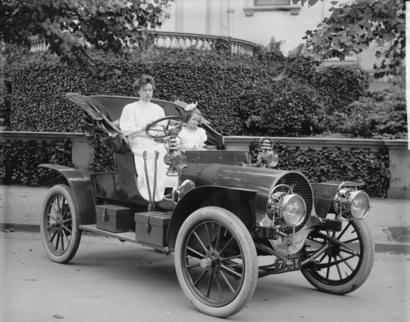
\includegraphics[width=\linewidth]{sample-franklin}
  \caption{1907 Franklin Model D roadster. Photograph by Harris \&
    Ewing, Inc. [Public domain], via Wikimedia
    Commons. (\url{https://goo.gl/VLCRBB}).}
  \Description{A woman and a girl in white dresses sit in an open car.}
\end{figure}


  % Some examples.  A paginated journal article \cite{Abril07}, an
  % enumerated journal article \cite{Cohen07}, a reference to an entire
  % issue \cite{JCohen96}, a monograph (whole book) \cite{Kosiur01}, a
  % monograph/whole book in a series (see 2a in spec. document)
  % \cite{Harel79}, a divisible-book such as an anthology or compilation
  % \cite{Editor00} followed by the same example, however we only output
  % the series if the volume number is given \cite{Editor00a} (so
  % Editor00a's series should NOT be present since it has no vol. no.),
  % a chapter in a divisible book \cite{Spector90}, a chapter in a
  % divisible book in a series \cite{Douglass98}, a multi-volume work as
  % book \cite{Knuth97}, a couple of articles in a proceedings (of a
  % conference, symposium, workshop for example) (paginated proceedings
  % article) \cite{Andler79, Hagerup1993}, a proceedings article with
  % all possible elements \cite{Smith10}, an example of an enumerated
  % proceedings article \cite{VanGundy07}, an informally published work
  % \cite{Harel78}, a couple of preprints \cite{Bornmann2019,
  %   AnzarootPBM14}, a doctoral dissertation \cite{Clarkson85}, a
  % master's thesis: \cite{anisi03}, an online document / world wide web
  % resource \cite{Thornburg01, Ablamowicz07, Poker06}, a video game
  % (Case 1) \cite{Obama08} and (Case 2) \cite{Novak03} and \cite{Lee05}
  % and (Case 3) a patent \cite{JoeScientist001}, work accepted for
  % publication \cite{rous08}, 'YYYYb'-test for prolific author
  % \cite{SaeediMEJ10} and \cite{SaeediJETC10}. Other cites might
  % contain 'duplicate' DOI and URLs (some SIAM articles)
  % \cite{Kirschmer:2010:AEI:1958016.1958018}. Boris / Barbara Beeton:
  % multi-volume works as books \cite{MR781536} and \cite{MR781537}. A
  % couple of citations with DOIs:
  % \cite{2004:ITE:1009386.1010128,Kirschmer:2010:AEI:1958016.1958018}. Online
  % citations: \cite{TUGInstmem, Thornburg01, CTANacmart}.
  % Artifacts: \cite{R} and \cite{UMassCitations}.

%%
%% The acknowledgments section is defined using the "acks" environment
%% (and NOT an unnumbered section). This ensures the proper
%% identification of the section in the article metadata, and the
%% consistent spelling of the heading.
\begin{acks}
To Alefiya, for the continual guidance and enthusiam all throughout
the project
\end{acks}

%%
%% The next two lines define the bibliography style to be used, and
%% the bibliography file.
\bibliographystyle{ACM-Reference-Format}
\bibliography{sample-base}

%%
%% If your work has an appendix, this is the place to put it.
\appendix
\end{document}
\endinput